\vspace{1em}
\scalebox{0.85}{
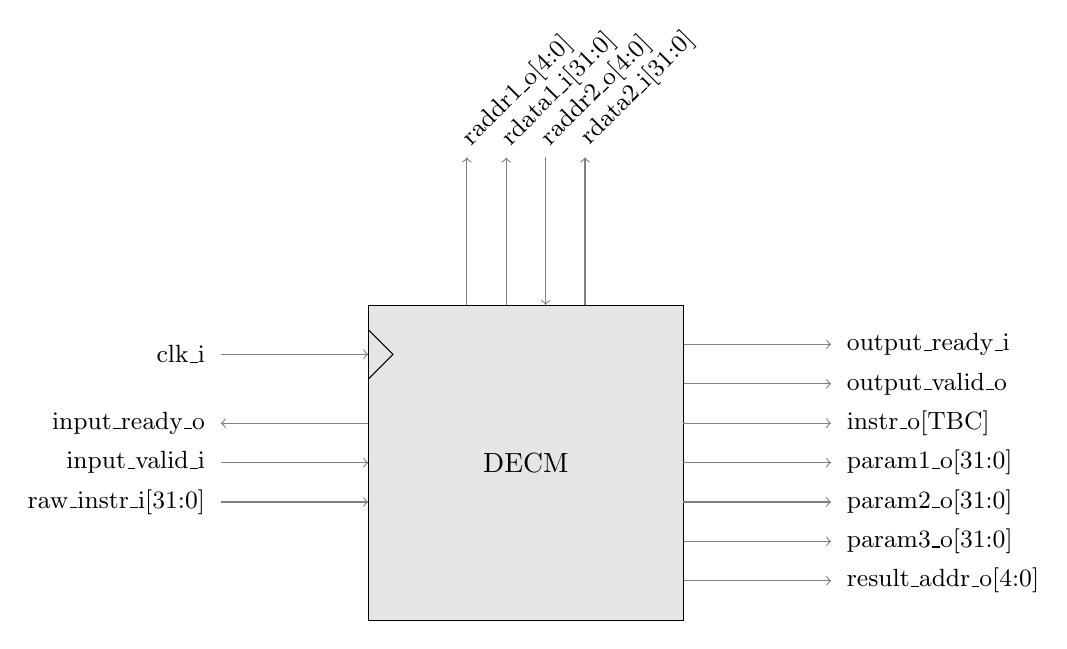
\begin{tikzpicture}[scale=1.25, draw=gray, inner sep=0, outer sep=0]
  \node[rectangle, draw=black,
    anchor=south,
    align=center,
    minimum height = 4cm,
    minimum width = 4cm,
    fill = gray!20] (block) at (0, 0) {DECM};

  \node (rport4) at (block.east) {};
  \node (rport3) at ([yshift=0.4cm]rport4.center) {};
  \node (rport2) at ([yshift=0.4cm]rport3.center) {};
  \node (rport1) at ([yshift=0.4cm]rport2.center) {};
  \node (rport5) at ([yshift=-0.4cm]rport4.center) {};
  \node (rport6) at ([yshift=-0.4cm]rport5.center) {};
  \node (rport7) at ([yshift=-0.4cm]rport6.center) {};
  \draw[<-] ([xshift=1.5cm]rport1.center) node[right=0.2cm, anchor=west]{\small output\_ready\_i} -- (rport1.center);
  \draw[<-] ([xshift=1.5cm]rport2.center) node[right=0.2cm, anchor=west]{\small output\_valid\_o} -- (rport2.center);
  \draw[<-] ([xshift=1.5cm]rport3.center) node[right=0.2cm, anchor=west]{\small instr\_o[TBC]} -- (rport3.center);
  \draw[<-] ([xshift=1.5cm]rport4.center) node[right=0.2cm, anchor=west]{\small param1\_o[31:0]} -- (rport4.center);
  \draw[<-] ([xshift=1.5cm]rport5.center) node[right=0.2cm, anchor=west]{\small param2\_o[31:0]} -- (rport5.center);
  \draw[<-] ([xshift=1.5cm]rport6.center) node[right=0.2cm, anchor=west]{\small param3\_o[31:0]} -- (rport6.center);
  \draw[<-] ([xshift=1.5cm]rport7.center) node[right=0.2cm, anchor=west]{\small result\_addr\_o[4:0]} -- (rport7.center);

  \node(uport2) at ([xshift=-0.2cm]block.north) {};
  \node(uport1) at ([xshift=-0.4cm]uport2.center) {};
  \node(uport3) at ([xshift=0.4cm]uport2.center) {};
  \node(uport4) at ([xshift=0.4cm]uport3.center) {};
  \draw[<-] ([yshift=1.5cm]uport1.center) node[above=0.2cm, anchor=west, rotate=45]{\small raddr1\_o[4:0]} -- (uport1.center);
  \draw[<-] ([yshift=1.5cm]uport2.center) node[above=0.2cm, anchor=west, rotate=45]{\small rdata1\_i[31:0]} -- (uport2.center);
  \draw[->] ([yshift=1.5cm]uport3.center) node[above=0.2cm, anchor=west, rotate=45]{\small raddr2\_o[4:0]} -- (uport3.center);
  \draw[<-] ([yshift=1.5cm]uport4.center) node[above=0.2cm, anchor=west, rotate=45]{\small rdata2\_i[31:0]} -- (uport4.center);

  \node (lport2) at (block.west) {};
  \node (lport1) at ([yshift=0.4cm]lport2.center) {};
  \node (lport3) at ([yshift=-0.4cm]lport2.center) {};

  \draw[<-] ([xshift=-1.5cm]lport1.center) node[left=0.2cm, anchor=east]{\small input\_ready\_o} -- (lport1.center);
  \draw[->] ([xshift=-1.5cm]lport2.center) node[left=0.2cm, anchor=east]{\small input\_valid\_i} -- (lport2.center);
  \draw[->] ([xshift=-1.5cm]lport3.center) node[left=0.2cm, anchor=east]{\small raw\_instr\_i[31:0]} -- (lport3.center);

  \node (clk) at ([yshift=-0.5cm]block.north west) {};
  \draw[->] ([xshift=-1.5cm]lport3.center |- clk.center) node[left=0.2cm, anchor=east]{\small clk\_i} -- (clk.center);
  % clk triangle
  \draw[-  , draw=black] ([yshift=0.25cm]clk.center) -- ([xshift=0.25cm]clk.center) -- ([yshift=-0.25cm]clk.center);
\end{tikzpicture}
}
